\documentclass[journal]{IEEEtran}
% DRAFT. Every number comes from paper/generated/, which paper/make_paper_data.py builds from results/raw/.
\usepackage{fontspec}
\setmainfont{texgyretermes}[Extension=.otf, UprightFont=*-regular, BoldFont=*-bold, ItalicFont=*-italic, BoldItalicFont=*-bolditalic]
\setmonofont{texgyrecursor}[Extension=.otf, UprightFont=*-regular, BoldFont=*-bold, ItalicFont=*-italic, BoldItalicFont=*-bolditalic]
\usepackage{cite}
\usepackage{amsmath,amssymb}
\usepackage{graphicx}
\usepackage{booktabs}
\usepackage{xcolor}
\usepackage{tikz}
\usetikzlibrary{positioning,arrows.meta,calc}
\usepackage{url}
% Generated by paper/make_paper_data.py. Do not edit.
\newif\ifsil
\siltrue
\newcommand{\AgreeHolds}{109}
\newcommand{\AgreeRuns}{144}
\newcommand{\AgreeSizes}{3, 4, 5}
\newcommand{\AgreeSpurious}{0}
\newcommand{\AgreeUnsound}{0}
\newcommand{\AgreeViolated}{35}
\newcommand{\ControlVerdict}{violated}
\newcommand{\DepthRule}{yes}
\newcommand{\DepthRuns}{14}
\newcommand{\EzeroAllExpected}{yes}
\newcommand{\EzeroChecks}{63}
\newcommand{\EzeroStatesOne}{674}
\newcommand{\EzeroStatesTwo}{1{,}224}
\newcommand{\EzeroStatesZero}{96}
\newcommand{\LiveHold}{12}
\newcommand{\LiveMax}{6}
\newcommand{\LiveMin}{3}
\newcommand{\LiveRuns}{12}
\newcommand{\MachineCpus}{8}
\newcommand{\MachineJava}{18.0.2}
\newcommand{\MachinePython}{3.14.4}
\newcommand{\PairRatioAtStop}{45{,}940}
\newcommand{\PairSecondsEdge}{3.57}
\newcommand{\PairSecondsNone}{1.93}
\newcommand{\PairStatesEdge}{148}
\newcommand{\PairStatesNone}{197}
\newcommand{\PredictCommit}{19423e3}
\newcommand{\RefineHold}{36}
\newcommand{\RefineRuns}{36}
\newcommand{\ReplayAll}{yes}
\newcommand{\ScaleAllFinishMax}{8}
\newcommand{\ScaleFaultBudget}{1}
\newcommand{\ScaleFinishedAtStop}{2}
\newcommand{\ScaleFirstNone}{10}
\newcommand{\ScaleFirstStop}{9}
\newcommand{\ScaleLongLimit}{1{,}200}
\newcommand{\ScalePeakRss}{2{,}218}
\newcommand{\ScaleSeeds}{3}
\newcommand{\ScaleShortLimit}{300}
\newcommand{\ScaleSlowestAtMax}{294.85}
\newcommand{\SevenDenseEdges}{6}
\newcommand{\SevenDenseStates}{190{,}288}
\newcommand{\SevenSparseEdges}{1}
\newcommand{\SevenSparseStates}{1{,}172{,}561}
\newcommand{\SilAllFalseAlarm}{0}
\newcommand{\SilAllMatchSafe}{27{,}837}
\newcommand{\SilAllMatchViol}{2{,}475}
\newcommand{\SilAllMiss}{0}
\newcommand{\SilAvailable}{yes}
\newcommand{\SilCampaigns}{5}
\newcommand{\SilCommit}{e593539}
\newcommand{\SilDistinctFalseAlarm}{0}
\newcommand{\SilDistinctMatchSafe}{19{,}442}
\newcommand{\SilDistinctMatchViol}{1{,}709}
\newcommand{\SilDistinctMiss}{0}
\newcommand{\SilRuns}{6{,}360}
\newcommand{\SilSOneDesigns}{LocalRollback}
\newcommand{\SilSOnePolicies}{late confirmation}
\newcommand{\SilSOneViol}{20}
\newcommand{\SilSameEnd}{6{,}360}
\newcommand{\SilSamePath}{6{,}360}
\newcommand{\SilScriptsSmall}{76}

\newcommand{\todo}[1]{\textcolor{red}{\textbf{TODO:} #1}}
\newcommand{\tla}{TLA\textsuperscript{+}}

\begin{document}

\title{Checking the Functional Safety of Multi-ECU Over-the-Air Update Campaigns: A \tla{} Model, a Pair Abstraction and Software-in-the-Loop Validation}

\author{Sravasti~Bose%
\thanks{S.~Bose is an independent researcher, Kolkata, India (e-mail: bosesravasti8@gmail.com).}%
\thanks{Draft, not yet submitted.}}

\markboth{Draft, \today}{}

\maketitle

\begin{abstract}
Over-the-air (OTA) updates in software-defined vehicles increasingly change several electronic control units (ECUs) in one campaign. If ECUs depend on one another's versions, a partial failure can leave a vehicle running an incompatible mix, even when every ECU recovers correctly on its own. We ask whether such campaign-level safety can be checked formally, and whether the model's predictions match an executable system. We model a dual-bank, coordinator-driven campaign in \tla{} and define four safety properties (compatibility at all times, a retained way back, all-or-nothing at campaign end, only verified images run) and one liveness property (the campaign finishes). The TLC model checker confirms them on a three-ECU campaign with up to two faults, and finds counterexamples in three flawed designs. One of them, rolling back only the failed ECU, violates compatibility after a single fault and passes every property without faults. Direct checking on one laptop finished for all generated campaigns up to \ScaleAllFinishMax{} ECUs and for none at \ScaleFirstNone{}. A pair abstraction reduces safety checking for any number of ECUs to two models of \PairStatesNone{} and \PairStatesEdge{} states, by a hand-written proof supported by mechanical refinement checks. \ifsil In a software-in-the-loop simulator with separate ECU processes, file-backed flash and process kills as power loss, \SilRuns{} fault-injected runs gave \SilAllMiss{} misses and \SilAllFalseAlarm{} false alarms against predictions frozen beforehand. Because model and simulator share an author and a schedule, this is evidence of consistency rather than independent validation. \else \todo{SIL results}\fi{} Hardware validation is future work.
\end{abstract}

\begin{IEEEkeywords}
Over-the-air update, software-defined vehicle, multi-ECU campaign, rollback, model checking, \tla{}, functional safety.
\end{IEEEkeywords}

\section{Introduction}

\IEEEPARstart{O}{ver-the-air} updates let a manufacturer change vehicle software after sale. When one feature spans several ECUs, the update becomes a \emph{campaign}: several ECUs must move to new versions that are only compatible with each other. Each ECU can protect itself with a dual-bank (A/B) layout, keeping its old image until the new one is confirmed. That protection is local. A campaign can still leave the vehicle in a state that no single ECU considers wrong, for example a brake controller running a version that needs a gateway version which has just been rolled back.

Regulation already asks for this. UN Regulation No.~156 requires manufacturers to identify interdependencies of the updated system with other systems, to confirm compatibility with the target vehicle's configuration before an update is issued, and to ensure the vehicle can restore its previous version, or reach a safe state, after a failed or interrupted update \cite{unr156}. ISO~24089 sets requirements for software update engineering, including for ECUs, but does not prescribe technologies \cite{iso24089}. Neither says how to show that a particular campaign design meets these goals.

Formal work on vehicle updates has so far concentrated on security. Uptane \cite{kuppusamy2016,kuppusamy2018}, which builds on TUF \cite{samuel2010}, has been analysed with CSP \cite{kirk2021,kirk2023}, Tamarin \cite{boureanu2023}, and a combination of the Kind~2 model checker with Tamarin, which found six new vulnerabilities \cite{lorch2024}. UniSUF has been verified in ProVerif \cite{hagen2026}. These analyses ask what an attacker can do. Uptane's designers also list a ``mixed-bundles'' attack, in which ECUs are made to install versions that must not run together, and note that partial installation can also happen by accident, for example when power runs out \cite{kuppusamy2016}. We study that hazard when no attacker is involved, and it is the update design itself, under faults, that leaves the vehicle in an incompatible or mixed state.

We ask two questions. \emph{Can functional safety of a multi-ECU campaign, including version dependencies, partial failure and rollback, be checked formally? And do the model's predictions match the behaviour of an executable implementation?}

Our contributions, each tied to one result:
\begin{enumerate}
\item A \tla{} model of a coordinator-driven A/B campaign, with four safety properties and one liveness property stated in plain language first (Section~\ref{sec:model}, Table~\ref{tab:props}).
\item A model-checking study that confirms the properties for a correct design and finds counterexamples in three flawed designs, including a rollback flaw invisible without faults (Section~\ref{sec:flaws}, Table~\ref{tab:e0}).
\item A measurement of where direct checking stops being practical, and a pair abstraction that covers safety for any number of ECUs, with a written proof and mechanical checks (Section~\ref{sec:scale}, Table~\ref{tab:scale}, Fig.~\ref{fig:scale}).
\item A software-in-the-loop (SIL) comparison of frozen model predictions against fault-injected runs (Section~\ref{sec:validation}, Tables~\ref{tab:confusion} and~\ref{tab:silbreak}).
\end{enumerate}
All code, raw results and run manifests are in the artifact repository \url{https://github.com/sravasti12/OTA-Campaign-Verfier-Research-Artifact}. Every number in this paper is generated from those raw files by a script.

\section{Background}
\label{sec:background}

\textbf{A/B updates.} Each ECU has two slots. It runs from one while the new image is written to the other, verifies it, switches to it for a trial, and confirms it if healthy. Until confirmation, switching back restores the old version.

\textbf{Campaigns.} A coordinator sequences downloads, activations and confirmations across ECUs. A dependency ``$x$ requires $d$'' means version~2 of $x$ may run only while $d$ runs version~2. On failure the coordinator rolls the campaign back.

\textbf{\tla{} and TLC.} \tla{} specifies a system as an initial-state predicate and a next-state relation, with temporal formulas for fairness and liveness \cite{lamport1994}. TLC is an explicit-state model checker for \tla{} \cite{yu1999}. It enumerates reachable states, checks invariants and temporal properties, and returns a shortest counterexample for a violated invariant. We use release v1.7.4 (TLC~2.19) \cite{tlaplus}. Apalache is a symbolic alternative \cite{konnov2019}, and TLAPS a proof system for \tla{} \cite{cousineau2012}. We used neither. \tla{} has been used on production distributed systems in industry \cite{newcombe2015}.

\section{Related Work}
\label{sec:related}

\begin{table*}[t]
\caption{Formal analyses of vehicle software updates that we located, and the object of this paper}
\label{tab:related}
\centering
\footnotesize
\begin{tabular}{@{}p{3.3cm}p{3.6cm}p{3.4cm}p{6.3cm}@{}}
\toprule
Work & Object & Technique & Properties \\
\midrule
Pedroza et al.\ \cite{pedroza2011} & Firmware update protocol between a communication unit and one ECU \cite{idrees2011} & AVATAR/SysML; ProVerif, with UPPAAL for safety & Security of the protocol (authenticity, confidentiality reported); framework also supports safety \\
Mahmood et al.\ \cite{mahmood2020,mahmood2022} & Uptane implementation & Threat assessment; attack-tree-based test generation & Security, by testing \\
Kirk et al.\ \cite{kirk2021,kirk2023} & Uptane & CSP models verified to generate tests & Security against a Dolev--Yao attacker \\
Mukherjee et al.\ \cite{mukherjee2021} & Uptane inside a TEE on COTS hardware & SAW (SAWScript) & Functional and logical inconsistencies in the code \\
Ponsard and Darquennes \cite{ponsard2021} & UpKit IoT update protocol & Tamarin & Firmware integrity, freshness of requests$^\ast$ \\
Boureanu \cite{boureanu2023} & Uptane 2.0 & Tamarin & Security and privacy \\
Lorch et al.\ \cite{lorch2024} & Uptane & Kind~2 with Tamarin & Security under nine threat models, including rollback (downgrade) attacks \\
Hagen et al.\ \cite{hagen2026} & UniSUF & ProVerif & Confidentiality, integrity, authenticity, freshness, order; liveness argued \\
\midrule
This paper & Multi-ECU A/B campaign with version dependencies & \tla{}/TLC, pair abstraction, SIL & Compatibility, retained way back, all-or-nothing at end, verified images only, termination, under faults and recovery \\
\bottomrule
\end{tabular}

\smallskip
\raggedright\scriptsize $^\ast$As described by Hagen et al.\ \cite{hagen2026}. We have read only the record of this paper, not its full text.
\end{table*}

\textbf{Security of update frameworks.} Table~\ref{tab:related} lists the formal analyses of vehicle software updates that we located. TUF \cite{samuel2010} and Uptane \cite{kuppusamy2016,kuppusamy2018} protect updates against compromised repositories and keys. Their analyses \cite{mahmood2020,mahmood2022,kirk2021,kirk2023,boureanu2023,lorch2024} and that of UniSUF \cite{hagen2026} all fix an attacker and ask what it can achieve. ``Rollback'' in that literature means a downgrade attack, in which an ECU is made to install an older, vulnerable image \cite{kuppusamy2016,lorch2024}. In this paper it means recovery after a failure. Hagen et al.\ name extension to multi-ECU and large-scale vehicular networks as future work, and point to assume--guarantee reasoning against state explosion \cite{hagen2026}. Uptane's director repository performs dependency resolution when choosing which images a vehicle installs \cite{kuppusamy2018}. That concerns which versions are \emph{selected}. Our properties concern which versions \emph{run} while a campaign executes and after it fails part way.

\textbf{Safety and the update process.} Pedroza et al.\ extended a safety-oriented modelling framework, which verifies safety properties with UPPAAL, to also cover security, and applied it to a firmware update protocol for a single in-car ECU \cite{pedroza2011,idrees2011}. Model checking has also been used for functional safety of automotive runtime logic, such as the arbitration of a fail-operational driving system, as evidence for ISO~26262 \cite{schmid2021}. Implementation-level work includes ScalOTA, a scalable OTA architecture with a formalized chain of trust \cite{shoker2023}, and an AUTOSAR-based firmware OTA implementation on a steering system \cite{mostafa2025}. Surveys cover OTA security for connected vehicles \cite{li2024} and the software-defined vehicle more broadly \cite{liotou2026}.

\textbf{Method.} Our pair abstraction is an over-approximating, safety-preserving abstraction in the sense of Clarke et al.\ \cite{clarke1994}. It checks a component against a stand-in environment, in the spirit of compositional model checking \cite{clarke1989}. Its refinement check, which maps full states to pair states, is a refinement mapping \cite{abadi1991}. Results showing that a small, fixed instance covers a whole family are known as cutoffs \cite{emerson1995}. Our proof is direct and uses none of those theorems. Trace validation links \tla{} specifications to implementations \cite{cirstea2024,howard2024}, a route to strengthening our SIL comparison.

\textbf{Gap.} In the sources we searched, none model-checks version compatibility across dependent ECUs under partial failure and recovery, or compares such a model against an executable implementation. We searched Crossref, arXiv, OpenAlex and the open web, and followed the reference lists of \cite{hagen2026,lorch2024}. We did not search the subscription databases IEEE Xplore and Scopus.

\section{Campaign Model and Properties}
\label{sec:model}

\subsection{Model}
The model, \texttt{OTACampaign.tla}, is parameterized by a set of ECUs, an acyclic dependency relation $D$, a fault budget $F$ and a design flag. Each ECU has an active version (1 or~2), the version held in its other slot, a stage, and a corruption flag. A shared variable records the campaign as \emph{run}, \emph{rollback}, \emph{committed} or \emph{aborted}. Fig.~\ref{fig:model} shows the steps.

\begin{figure}[t]
\centering
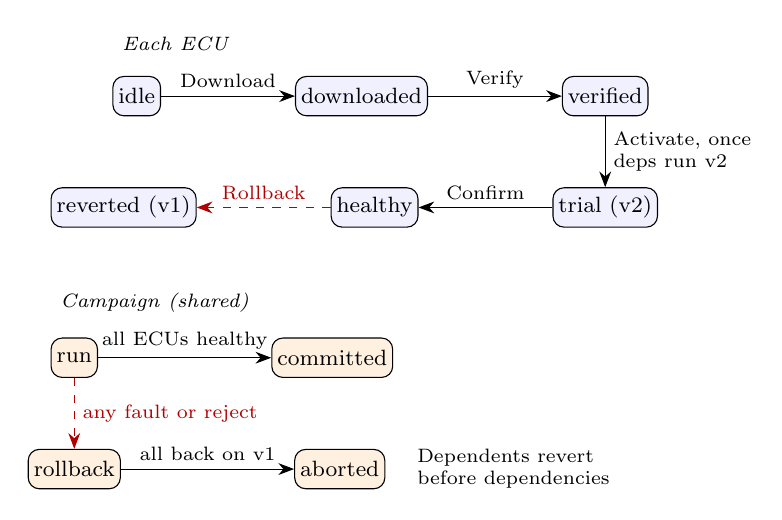
\begin{tikzpicture}[node distance=9mm and 17mm, font=\footnotesize,
  st/.style={draw, rounded corners, minimum height=5mm, inner sep=2pt, fill=blue!6},
  cp/.style={draw, rounded corners, minimum height=5mm, inner sep=2pt, fill=orange!12},
  lb/.style={font=\scriptsize, inner sep=1pt, outer sep=2pt},
  ar/.style={-{Stealth[length=2mm]}}, fl/.style={-{Stealth[length=2mm]}, dashed, red!70!black}]
\node[font=\scriptsize\itshape] (h1) {Each ECU};
\node[st, below=2mm of h1.south west, anchor=north west] (idle) {idle};
\node[st, right=of idle] (dl) {downloaded};
\node[st, right=of dl] (ver) {verified};
\node[st, below=of ver] (tr) {trial (v2)};
\node[st, left=of tr] (ok) {healthy};
\node[st, left=of ok] (rev) {reverted (v1)};
\draw[ar] (idle) -- node[lb, above]{Download} (dl);
\draw[ar] (dl) -- node[lb, above]{Verify} (ver);
\draw[ar] (ver) -- node[lb, right, align=left]{Activate, once\\deps run v2} (tr);
\draw[ar] (tr) -- node[lb, above]{Confirm} (ok);
\draw[fl] (ok) -- node[lb, above]{Rollback} (rev);
\node[font=\scriptsize\itshape, below=7mm of rev.south west, anchor=north west] (h2) {Campaign (shared)};
\node[cp, below=2mm of h2.south west, anchor=north west] (run) {run};
\node[cp, right=22mm of run] (com) {committed};
\node[cp, below=of run] (rb) {rollback};
\node[cp, right=22mm of rb] (ab) {aborted};
\draw[ar] (run) -- node[lb, above]{all ECUs healthy} (com);
\draw[fl] (run) -- node[lb, right]{any fault or reject} (rb);
\draw[ar] (rb) -- node[lb, above]{all back on v1} (ab);
\node[lb, align=left, right=3mm of ab] {Dependents revert\\before dependencies};
\end{tikzpicture}
\caption{The campaign model. Top: one ECU's stages. Bottom: the shared campaign state. Dashed: a fault and the rollback it starts. Faults are download failure, corrupt download, trial failure and vehicle-wide power loss, and each uses one unit of the budget $F$.}
\label{fig:model}
\end{figure}

\textbf{Correct design.} An ECU activates only after the ECUs it depends on run version~2. On any failure the campaign enters rollback, and every ECU on version~2 reverts, dependents before their dependencies. The campaign then ends as aborted.

\textbf{Faults.} Download failure, corrupt download, trial failure and vehicle-wide power loss, which discards unverified downloads and starts rollback. Power loss may also strike during rollback, which then resumes.

\textbf{Flawed designs.} One flag changes one decision. \texttt{LocalRollback} reverts only the ECU that failed. \texttt{EarlyErase} discards the old image on activation to free flash. \texttt{SkipVerify} accepts any downloaded image.

\textbf{Simplifications.} Steps are atomic. The campaign state is one durable, shared variable, so there is no message loss or delay between coordinator and ECUs. There are no timeouts or retries. Each ECU has two versions. These limits recur in Section~\ref{sec:threats}.

\subsection{Properties}
The properties were written in plain English before the model. Table~\ref{tab:props} gives each one and the wording the results support.

\begin{table}[t]
\caption{Properties checked}
\label{tab:props}
\centering
\footnotesize
\begin{tabular}{@{}p{0.5cm}p{3.6cm}p{3.6cm}@{}}
\toprule
& Formal statement & What it does \emph{not} claim \\
\midrule
S1 & For every $(x,d)\in D$: $x$ runs v2 $\Rightarrow$ $d$ runs v2, in every reachable state & Version ranges; dependencies among three or more ECUs \\
S2 & Before commit, every ECU running v2 holds v1 in its other slot & That the kept image boots \\
S3 & Once committed or aborted, all ECUs run v1 or all run v2 & Consistency at intermediate states \\
S4 & No ECU runs an image flagged corrupt & Any security property \\
L1 & Under weak fairness and at most $F$ faults, the campaign reaches committed or aborted & Termination with unbounded faults or timeouts \\
\bottomrule
\end{tabular}
\end{table}

\section{Model Checking the Designs}
\label{sec:flaws}

We checked a three-ECU campaign (gateway, brake, infotainment; brake requires gateway) for all four designs and five properties at fault budgets 0, 1 and~2, plus three sanity checks: TLC was asked to find a commit, an abort and a real rollback in the correct design, so that a pass cannot come from a model that does nothing. All \EzeroChecks{} checks matched verdicts recorded before the first run (at budget~2). The correct design was fully explored with \EzeroStatesZero{}, \EzeroStatesOne{} and \EzeroStatesTwo{} distinct states at budgets 0, 1 and~2. Table~\ref{tab:e0} gives the verdicts.

\begin{table}[t]
\caption{Verdicts on the three-ECU campaign at fault budget 2. Parentheses: smallest budget at which the violation appears}
\label{tab:e0}
\centering
\scriptsize
\setlength{\tabcolsep}{2.5pt}
\begin{tabular}{@{}lccccc@{}}
\toprule
Design & S1 & S2 & S3 & S4 & L1 \\
\midrule
Correct & holds & holds & holds & holds & holds \\
LocalRollback & \textbf{violated} (1) & holds & \textbf{violated} (1) & holds & holds \\
EarlyErase & holds & \textbf{violated} (0) & holds & holds & \textbf{violated} (1) \\
SkipVerify & holds & holds & holds & \textbf{violated} (1) & holds \\
\bottomrule

\end{tabular}
\end{table}

\begin{table}[t]
\caption{Shortest counterexamples, at the smallest fault budget that produces each violation}
\label{tab:cex}
\centering
\footnotesize
\setlength{\tabcolsep}{3pt}
\begin{tabular}{@{}llrrlrc@{}}
\toprule
Design & Prop. & Faults & States & Ending & Explored & Replayed \\
\midrule
LocalRollback & S1 & 1 & 9 & finite & 406 & yes \\
LocalRollback & S3 & 1 & 6 & finite & 158 & yes \\
EarlyErase & S2 & 0 & 4 & finite & 11 & yes \\
EarlyErase & L1 & 1 & 11 & stuttering & 437 & yes \\
SkipVerify & S4 & 1 & 4 & finite & 56 & yes \\
\bottomrule

\end{tabular}

\smallskip
\raggedright\scriptsize States: length of the trace. Ending: \emph{stuttering} means the trace ends in a state the campaign never leaves. Explored: distinct states TLC visited before stopping. Replayed: the trace was re-executed step by step by a separate Python checker that does not use TLC.
\end{table}

Table~\ref{tab:cex} lists the counterexamples. Each one was replayed by an independent checker (all replayed: \ReplayAll).

\textbf{Rolling back only the failed ECU.} Gateway and brake both activate version~2. Gateway then fails its health check, and only gateway reverts. Brake keeps running version~2 against a gateway on version~1, violating S1, and the campaign ends as aborted with the mix in place. With no faults this design passes every property, so nominal testing would not reveal it.

\textbf{Erasing early.} With no faults at all, an ECU that activates version~2 has no way back, violating S2. With one corrupt download detected late, two ECUs cannot revert, and the campaign stays in rollback forever (L1). This design ``holds'' S3 only because the stuck campaign never ends, so S3 and L1 are needed together.

\textbf{Skipping verification.} A corrupt image runs after one fault (S4). This variant exists to show that S4 can fail.

Every property was violated by at least one design, which shows that each one can fail in this model.

\section{Scalability and Abstraction}
\label{sec:scale}

\subsection{Direct checking}
We generated acyclic dependency graphs with a seeded generator, \ScaleSeeds{} graphs per size, and checked S1--S4 together with TLC at a fault budget of \ScaleFaultBudget{} (1 worker, 4\,GB heap) on one laptop with \MachineCpus{} logical CPUs and Java~\MachineJava. Sizes up to 10 ran with a limit of \ScaleLongLimit\,s, and sizes 20 and 50 with \ScaleShortLimit\,s. We call checking \emph{practical} when TLC finishes within the limit. This is our definition, tied to this machine.

\begin{table}[t]
\caption{Direct checking of S1--S4, fault budget \ScaleFaultBudget}
\label{tab:scale}
\centering
\footnotesize
\setlength{\tabcolsep}{3pt}
\begin{tabular}{@{}rcrrrr@{}}
\toprule
ECUs & Finished & Limit (s) & Median states & Median time (s) & Peak MB \\
\midrule
5 & 3 of 3 & 1{,}200 & 23{,}979 & 4.94 & 365 \\
6 & 3 of 3 & 1{,}200 & 47{,}120 & 6.58 & 629 \\
7 & 3 of 3 & 1{,}200 & 275{,}083 & 13.10 & 1{,}540 \\
8 & 3 of 3 & 1{,}200 & 4{,}500{,}928 & 274.89 & 1{,}914 \\
9 & 2 of 3 & 1{,}200 & 9{,}050{,}115$^\dagger$ & 662.59 & 2{,}218 \\
10 & 0 of 3 & 1{,}200 & -- & -- & 2{,}189 \\
20 & 0 of 3 & 300 & -- & -- & 1{,}686 \\
50 & 0 of 3 & 300 & -- & -- & 1{,}540 \\
\bottomrule

\end{tabular}

\smallskip
\raggedright\scriptsize $^\dagger$Finished runs only, so the value understates the true median. Runs that stopped report no totals.
\end{table}

\begin{figure*}[t]
\centering
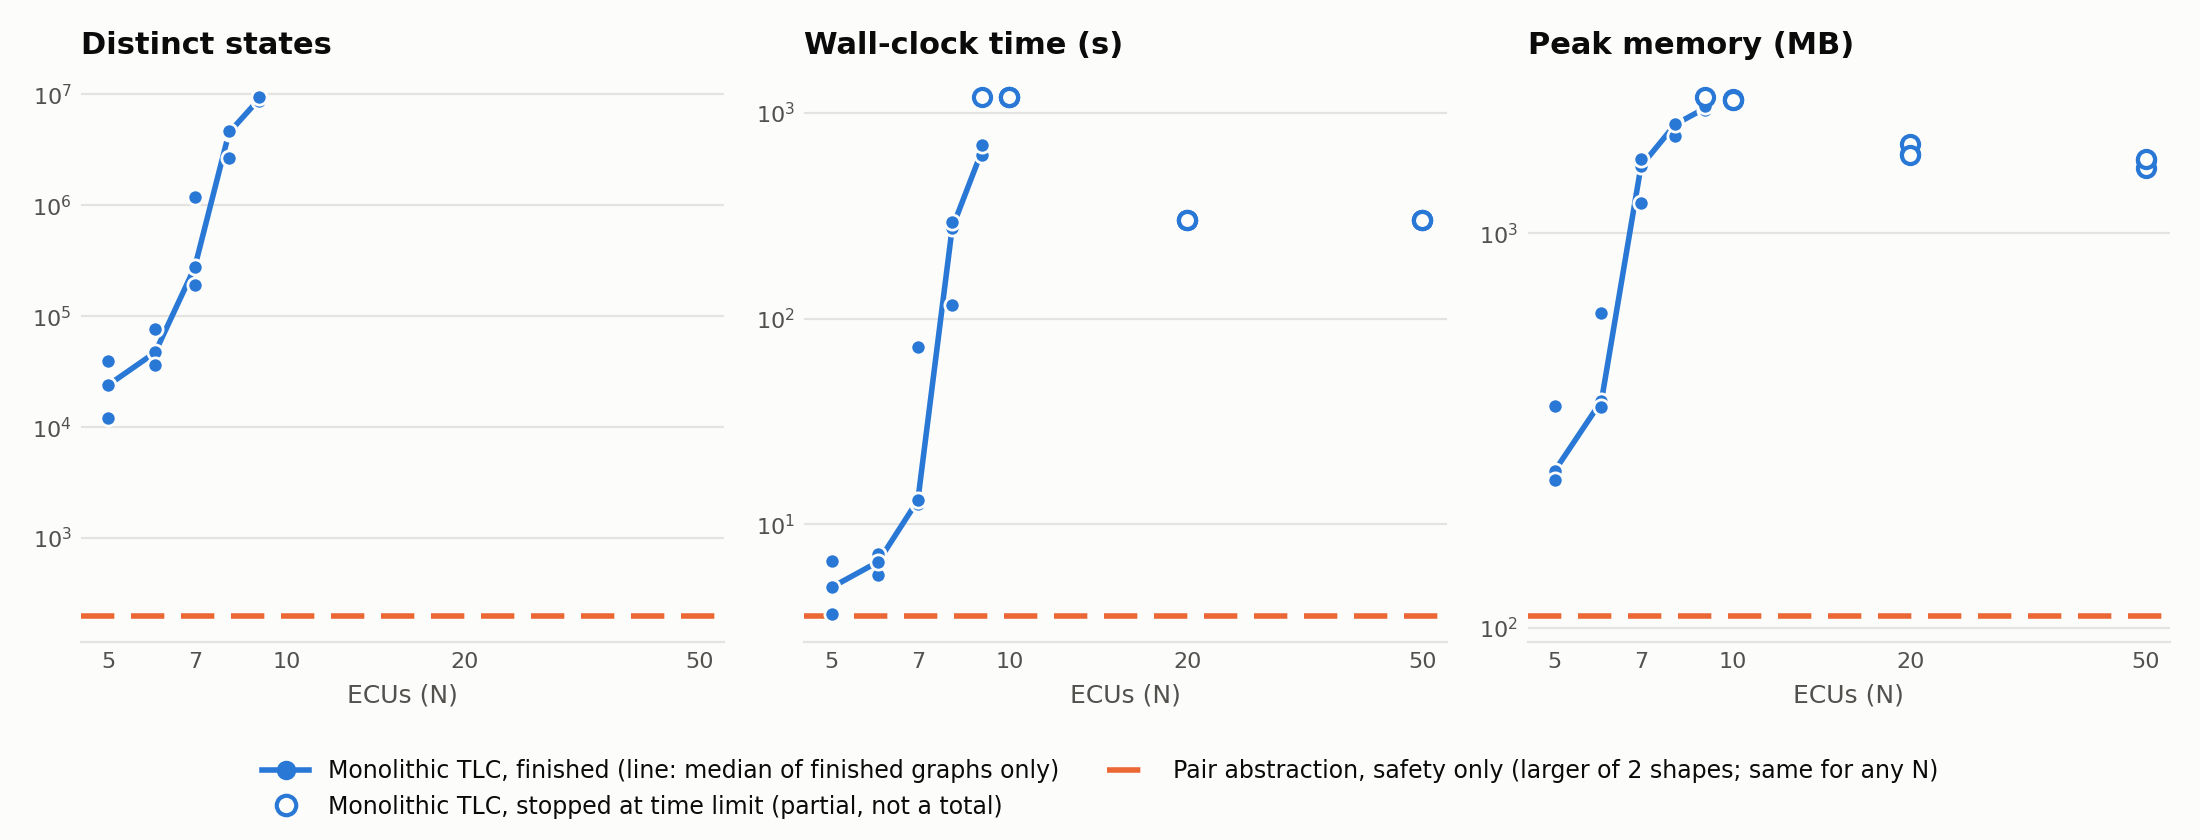
\includegraphics[width=\textwidth]{../results/scaling.png}
\caption{Direct checking of S1--S4 against the number of ECUs (log-log). Hollow markers: runs stopped at the time limit, whose values are not totals. Dashed: the larger of the two pair models, whose cost does not depend on the number of ECUs.}
\label{fig:scale}
\end{figure*}

All graphs finished up to \ScaleAllFinishMax{} ECUs, \ScaleFinishedAtStop{} of 3 at \ScaleFirstStop{}, and none at \ScaleFirstNone{} or above (Table~\ref{tab:scale}, Fig.~\ref{fig:scale}). Time, not memory, was the limit: peak memory stayed at or below \ScalePeakRss\,MB. With a five-minute budget the boundary would be \ScaleAllFinishMax{} ECUs, as the slowest run there took \ScaleSlowestAtMax\,s. The graph mattered as much as the size. At 7 ECUs, a graph with \SevenSparseEdges{} edge reached \SevenSparseStates{} states and one with \SevenDenseEdges{} edges \SevenDenseStates{}, because fewer dependencies allow more interleavings. Three graphs per size are too few to fit a growth rate, so we report none. The liveness property L1 was checked directly only at \LiveMin{} to \LiveMax{} ECUs, and held in all \LiveRuns{} runs (Table~\ref{tab:live}).

\begin{table}[t]
\caption{Direct checking of liveness L1 (correct design, fault budget \ScaleFaultBudget). Values per graph, seeds 1 / 2 / 3}
\label{tab:live}
\centering
\footnotesize
\setlength{\tabcolsep}{3pt}
\begin{tabular}{@{}rllrc@{}}
\toprule
ECUs & Edges & Distinct states & Max time (s) & L1 holds \\
\midrule
3 & 1 / 1 / 2 & 674 / 674 / 529 & 1.79 & 3 of 3 \\
4 & 2 / 4 / 1 & 3{,}405 / 1{,}694 / 4{,}358 & 2.34 & 3 of 3 \\
5 & 0 / 2 / 4 & 39{,}379 / 23{,}979 / 12{,}075 & 6.43 & 3 of 3 \\
6 & 7 / 5 / 5 & 47{,}120 / 36{,}025 / 76{,}484 & 13.71 & 3 of 3 \\
\bottomrule

\end{tabular}
\end{table}

\subsection{Pair abstraction}
Each safety property mentions at most two ECUs. We therefore check two ECUs $\{a,b\}$ against an environment that may fail at any time. The pair model keeps the two ECUs' variables and the campaign state, drops the fault counter, and adds one action, \emph{EnvFail}, which moves the campaign from run to rollback. An abstraction function $\alpha$ restricts a full state to the pair.

\textbf{Theorem 1.} Fix a design. If S1--S4 hold in both pair shapes (no edge, and one edge $a$ requires $b$), then S1--S4 hold in every reachable state of the full model for every finite set of at least two ECUs, every acyclic $D$ and every fault budget.

\emph{Proof sketch.} $\alpha$ maps the initial state to the pair's initial state. Every full step maps to a pair step or a stutter. Steps of ECUs outside the pair either leave the pair unchanged or start rollback, matched by \emph{EnvFail}. Steps inside the pair have the same effect and weaker guards in the pair model, since the pair sees only its own dependencies and has no fault budget. By induction, $\alpha$ of every reachable full state is reachable in a pair model. Renaming reduces every pair to the two shapes. S1, S2 and S4 then transfer directly. For S3, equal versions on every pair imply equal versions on all ECUs. The full proof is in the artifact. It has \emph{not} been machine-checked, for example in TLAPS \cite{cousineau2012}, or independently reviewed, and we present it as a proof sketch.

The abstraction over-approximates \cite{clarke1994}, so a pair ``violated'' verdict is only a warning, while ``holds'' is a guarantee. It says nothing about L1. For L1 we give only an informal argument, which needs acyclic $D$, and treat it as such.

\textbf{Cost.} The correct design's two pair models have \PairStatesNone{} and \PairStatesEdge{} distinct states and took \PairSecondsNone\,s and \PairSecondsEdge\,s, independent of the number of ECUs. At \ScaleFirstStop{} ECUs, the median finished direct run had about \PairRatioAtStop{} times as many states as the larger pair model. Table~\ref{tab:pair} gives the pair models for every design. For each design, the pair models flag exactly the safety properties that the three-ECU campaign violates (Table~\ref{tab:e0}). L1 is outside the pair models, and \texttt{LocalRollback}'s S1 warning appears only in the shape with an edge, as S1 constrains only dependent pairs.

\begin{table}[t]
\caption{Pair models: distinct states (from a property that holds) and properties violated}
\label{tab:pair}
\centering
\footnotesize
\setlength{\tabcolsep}{4pt}
\begin{tabular}{@{}llrl@{}}
\toprule
Design & Shape & States & Violated \\
\midrule
Correct & none & 197 & -- \\
Correct & edge & 148 & -- \\
LocalRollback & none & 193 & S3 \\
LocalRollback & edge & 149 & S1 S3 \\
EarlyErase & none & 141 & S2 \\
EarlyErase & edge & 117 & S2 \\
SkipVerify & none & 407 & S4 \\
SkipVerify & edge & 289 & S4 \\
\bottomrule

\end{tabular}
\end{table}

\begin{table}[t]
\caption{Pair prediction against full-model verdict, \AgreeSizes{} ECUs, fault budget 2, S1--S4}
\label{tab:agree}
\centering
\footnotesize
\setlength{\tabcolsep}{4pt}
\begin{tabular}{@{}lrrrr@{}}
\toprule
Design & Both hold & Both violated & Unsound & Spurious \\
\midrule
Correct & 36 & 0 & 0 & 0 \\
LocalRollback & 19 & 17 & 0 & 0 \\
EarlyErase & 27 & 9 & 0 & 0 \\
SkipVerify & 27 & 9 & 0 & 0 \\
\bottomrule

\end{tabular}
\end{table}

\textbf{Mechanical checks.} These test the proof's lemmas on finite instances. They support the proof but do not replace it.
(i)~Refinement: TLC checked that the full model refines the pair model through $\alpha$ for every ECU pair, in \RefineHold{} of \RefineRuns{} runs on small generated campaigns over all four designs.
(ii)~Negative control: with \emph{EnvFail} disabled, the same check was \ControlVerdict, so the check can detect a broken abstraction.
(iii)~Agreement: on \AgreeSizes{} ECUs at a fault budget of 2, pair predictions matched full-model verdicts in all \AgreeRuns{} comparisons (\AgreeHolds{} both hold, \AgreeViolated{} both violated), with \AgreeUnsound{} unsound and \AgreeSpurious{} spurious results (Table~\ref{tab:agree}). That zero applies only to these instances.

\section{Validation Against a Software-in-the-Loop Simulator}
\label{sec:validation}

\subsection{Setup}
The SIL runs each ECU as a separate operating-system process with file-backed slots and a durable boot record. Power loss kills every ECU process at once and restarts them from disk. Verification compares a SHA-256 digest of the image, and a corrupt download really corrupts bytes. The coordinator keeps its campaign state in a durable file and is rebuilt from it after power loss. An oracle judges S1--S4 from the bytes on disk after every step, not from what the coordinator believes. L1 is judged in finite runs as ``the campaign has ended''. The SIL was written from the plain-language design and imports nothing from the model or its tooling. A test enforces this.

\textbf{Campaigns and faults.} The SIL runs \SilCampaigns{} campaigns (Table~\ref{tab:silcamp}): the three-ECU campaign, three generated 5-ECU campaigns and one 10-ECU campaign. Each runs under three schedules (batch, rolling, and late confirmation, where trial periods overlap) and all four designs. Fault scripts cover no fault, every applicable single fault at every step, and, for campaigns of at most five ECUs, each single fault followed by a power loss one or three steps later. For the three-ECU campaign this gives \SilScriptsSmall{} scripts per schedule and design.

\begin{table}[t]
\caption{SIL campaigns. Runs = scripts $\times$ 3 schedules $\times$ 4 designs}
\label{tab:silcamp}
\centering
\footnotesize
\setlength{\tabcolsep}{2.5pt}
\begin{tabular}{@{}lrrrrrr@{}}
\toprule
Campaign & ECUs & Edges & Runs & Paths & Viol. & Mismatch \\
\midrule
Three-ECU & 3 & 1 & 912 & 597 & 321 & 0 \\
5 ECUs, seed 1 & 5 & 0 & 1{,}488 & 989 & 572 & 0 \\
5 ECUs, seed 2 & 5 & 2 & 1{,}488 & 989 & 578 & 0 \\
5 ECUs, seed 3 & 5 & 4 & 1{,}488 & 989 & 578 & 0 \\
10 ECUs, seed 1 & 10 & 9 & 984 & 864 & 426 & 0 \\
\bottomrule

\end{tabular}

\smallskip
\raggedright\scriptsize Paths: distinct predicted action sequences per design and schedule. Viol.: property cells where a violation was predicted and observed. Mismatch: misses plus false alarms.
\end{table}

\textbf{Predictions.} A scripted version of the model, pinned to the same schedule and fault script, predicted for each run the violated properties, the action path and the end state. \ifsil The predictions were generated from commit \texttt{\PredictCommit} and committed as \texttt{\SilCommit}, and the SIL then ran from that same commit. \fi

\subsection{Results}
\ifsil
Each run and property is one cell: a violation predicted and observed (match), neither (match safe), observed but not predicted (miss), or predicted but not observed (false alarm). S1 cells in the campaign without edges are left out, because S1 cannot be violated there. Many fault scripts lead to the same run, so we also count distinct (campaign, design, schedule, path, verdict) combinations.

Over \SilRuns{} runs, there were \SilAllMatchViol{} matched violations, \SilAllMatchSafe{} matched safe cells, \SilAllMiss{} misses and \SilAllFalseAlarm{} false alarms (distinct runs: \SilDistinctMatchViol, \SilDistinctMatchSafe, \SilDistinctMiss{} and \SilDistinctFalseAlarm). The predicted action path matched the observed one in \SilSamePath{} runs and the end state in \SilSameEnd{} (Table~\ref{tab:confusion}).
\else
\todo{SIL results: the run had not finished when this draft was built.}
\fi

\begin{table}[t]
\caption{Model predictions against SIL observations, per property. All runs (distinct runs in parentheses)}
\label{tab:confusion}
\centering
\footnotesize
\setlength{\tabcolsep}{3pt}
\begin{tabular}{@{}lrrrr@{}}
\toprule
& Match (viol.) & Match (safe) & Miss & False alarm \\
\midrule
S1 & 20 (15) & 4{,}852 (3{,}424) & 0 (0) & 0 (0) \\
S2 & 846 (577) & 5{,}514 (3{,}851) & 0 (0) & 0 (0) \\
S3 & 676 (453) & 5{,}684 (3{,}975) & 0 (0) & 0 (0) \\
S4 & 102 (102) & 6{,}258 (4{,}326) & 0 (0) & 0 (0) \\
L1 & 831 (562) & 5{,}529 (3{,}866) & 0 (0) & 0 (0) \\
\bottomrule

\end{tabular}
\end{table}

\begin{table}[t]
\caption{Model predictions against SIL observations, by design and by schedule (all runs, all properties)}
\label{tab:silbreak}
\centering
\footnotesize
\setlength{\tabcolsep}{3pt}
\begin{tabular}{@{}lrrrr@{}}
\toprule
& Match (viol.) & Match (safe) & Miss & False alarm \\
\midrule
Correct & 0 & 7{,}578 & 0 & 0 \\
LocalRollback & 696 & 6{,}882 & 0 & 0 \\
EarlyErase & 1{,}677 & 5{,}901 & 0 & 0 \\
SkipVerify & 102 & 7{,}476 & 0 & 0 \\
\midrule
Batch & 570 & 9{,}534 & 0 & 0 \\
Rolling & 1{,}353 & 8{,}751 & 0 & 0 \\
Late confirmation & 552 & 9{,}552 & 0 & 0 \\
\bottomrule

\end{tabular}
\end{table}

The correct design produced no violation in any run, and every flawed design produced violations that the model had predicted (Table~\ref{tab:silbreak}). All \SilSOneViol{} S1 violations came from design \texttt{\SilSOneDesigns} under schedule ``\SilSOnePolicies''. That is the only schedule in which a dependency can still be in its trial period, and so able to fail, after its dependent has activated. This is why \texttt{LocalRollback}'s S1 flaw needs a particular schedule to show.

\textbf{How to read this.} Agreement is the expected outcome when two implementations of one design follow the same schedule. The comparison shows that the model and an executable, process-level implementation agree on these campaigns and faults, including after real process kills and real hash checks. It does not show that the model captures failure modes the SIL cannot produce, such as torn writes, because the SIL injects only the model's fault kinds. A power cut during a write is the one fault that is lower-level in the SIL than in the model, where it maps to a power loss at that step.

\section{Discussion and Threats to Validity}
\label{sec:threats}

\textbf{Construct.} The properties are narrower than ``safe update''. S3 is checked only at campaign end, S2 does not establish that the kept image boots, and S4 is not a security property (Table~\ref{tab:props}). Each ECU has two versions, and dependencies are pairwise.

\textbf{Model scope.} Steps are atomic, and the campaign state is shared and durable, with no message loss, delay, timeouts or retries. The pair-abstraction proof depends on the shared campaign variable, and message loss would add behaviours it does not cover.

\textbf{Internal.} The same author wrote the model, the flawed designs, the SIL and the fault scripts, and the flaws were chosen, not found. Agreement between model and SIL is therefore weak evidence of the model's accuracy. An independent update client and fault kinds outside the model, such as torn writes and message loss, would strengthen it. We leave both to future work.

\textbf{Proof.} Theorem~1 is a hand proof, checked by us and by finite mechanical tests only. L1 beyond \LiveMax{} ECUs rests on an argument, not a proof.

\textbf{Measurement.} Each scaling configuration ran once on one Windows laptop, so timings have no variance estimate. Our other work overlapped the timings at 5 and 6 ECUs, though not their state counts. Limits of \ScaleShortLimit\,s at 20 and 50 ECUs show only that TLC did not finish in that time. A server, longer limits, multi-worker TLC or Apalache \cite{konnov2019} would move the boundary. The fault budget was \ScaleFaultBudget{} in the scaling runs.

\textbf{External.} Nothing here was run on vehicle hardware, real ECU flash, CAN, or AUTOSAR software. A Raspberry Pi testbed with relay-switched power cuts is designed but not built, and hardware results are future work.

\textbf{Standards.} UN Regulation No.~156 asks that interdependencies be identified, compatibility be confirmed before release, and the vehicle be able to return to its previous version or a safe state after a failed or interrupted update \cite{unr156}. Our properties S1--S3 are one way to make the last of these precise for a campaign. We draw no conclusion about compliance or certification, which concern a manufacturer's processes as well as its designs. We have read only the scope of ISO~24089 \cite{iso24089}, not its requirements.

\textbf{Literature search.} The related-work search did not cover IEEE Xplore or Scopus (Section~\ref{sec:related}), so relevant work indexed only there may be missing.

\section{Conclusion}
A dual-bank layout makes each ECU recoverable, but not the vehicle. A small \tla{} model with five properties separates a correct campaign from three plausible mistakes. One of them, rolling back only the failed ECU, is invisible without faults. Direct model checking reached \ScaleAllFinishMax{} ECUs on a laptop. A pair abstraction moves safety checking to two small models for any number of ECUs, resting on a hand proof that still needs independent review. \ifsil A process-level simulator agreed with frozen model predictions in every run we tried, which shows consistency, not independent validation. \fi{}Next steps are independent fault sources, message-level coordination, and hardware power cuts.

\section*{Artifact}
Model, scripts, raw results with manifests (commit, uncommitted files, seed, environment and SHA-256 of every output) and the generator for every number in this paper: \url{https://github.com/sravasti12/OTA-Campaign-Verfier-Research-Artifact}.

\bibliographystyle{IEEEtran}
\bibliography{refs}

\end{document}
